
\section{Ablation Studies}
\label{sec:analysis}

Here we ablate various
context window and architecture components of RT,
seeking to understand their role in
enabling zero-shot transfer and
contrasting that with their impact on fine-tuning.

\subsection{Context Window Ablations}
\label{sec:context_ablation}




\paragraph{Setup.}
In Table~\ref{tab:ctx_ablations},
we investigate the impact of 
shuffling column and table names,
removing past task rows which refer to the target entity
(\textbf{self labels} in short)
and removing task rows from other entities
(\textbf{other labels}).
We use the same pretrained checkpoints as in \S~\ref{sec:experiments}.
We provide a breakdown of self and other labels in $1024$ cell contexts
in Tab.~\ref{tab:context_breakdown}.

\begin{figure}[t]
\centering
\begin{minipage}[b]{0.43\textwidth}
    \centering
    \scriptsize
    \begin{tabular}{lrrrr}
    \toprule
    \multirow{2}{*}{Ablated $\downarrow$}
    & \multicolumn{2}{c}{Zero-shot}
    & \multicolumn{2}{c}{Fine-tuned} \\
    \cmidrule{2-3} \cmidrule{4-5}
    & clf
    & reg
    & clf
    & reg \\
    \midrule
    none & $70.1$ & $22.8$ & $77.2$ & $33.2$ \\
    col names & \cellcolor{red!5} $69.5$ & \cellcolor{red!15} $20.5$ & \cellcolor{green!5} $77.5$ & \cellcolor{red!0} $33.2$ \\
    self labels & \cellcolor{red!90} $53.8$ & \cellcolor{red!90} $-5.5$ & \cellcolor{red!1} $77.1$ & \cellcolor{red!30} $26.7$ \\
    other labels & \cellcolor{green!2} $70.6$ & \cellcolor{green!1} $22.9$ & \cellcolor{green!1} $77.4$ & \cellcolor{red!10} $31.0$ \\
    \bottomrule
    \end{tabular}
    \captionof{table}{
    Mean AUROC (\%) and R$^2$ (\%) on ablating context window components
    for classification (clf) and regression (reg) tasks. %respectively.
    Individual numbers are in App.~\ref{app:cont_ablations}.
    }
    \label{tab:ctx_ablations}
\end{minipage}
\hfill
\begin{minipage}[b]{0.54\textwidth}
% \begin{wrapfigure}{r}{\linewidth}
% \vspace{-12pt}
\centering
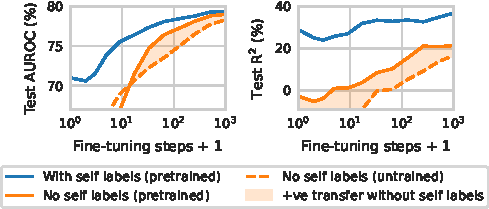
\includegraphics[width=\linewidth]{auto-figures/transfer-wo-self-labels.pdf}
\caption{
Pretrained RT shows transfer even without self labels.
% especially after some fine-tuning.
Setup is same as in Fig.~\ref{fig:learn-avg}.
}
\label{fig:transfer-wo-self-labels}
\end{minipage}%
\end{figure}

\paragraph{Observations.}
% 1)
We find that zero-shot transfer is driven primarily by the model’s ability to leverage past labels of the target entity.
From EntityMean baseline results in \S~\ref{sec:experiments},
we know that RT is learning more complex functions than averaging
self labels.
Fig.~\ref{fig:transfer-wo-self-labels} investigates whether the model learns other transferable patterns besides self label ones.
The positive transfer regions in the plots establish that this is indeed the case,
but self labels do constitute the dominant share of transfer from pretraining
even during initial steps of fine-tuning.
% 2)
Second, we find that the model indeed leverages table/column names
for zero-shot transfer, as wrong names lead to consistent degradation.
% 3)
After full fine-tuning, context ablations have little effect,
except that removing self labels significantly degrades performance on regression tasks.










\subsection{Relational Attention Layer Ablations}
\label{sec:layer_ablation}

\paragraph{Setup.} 
In Tab.~\ref{tab:attention_ablations}, we report the effect of removing column, feature, neighbor, or full attention layers on regression tasks. Classification tasks (App.~\ref{app:ablations}) showed minor differences.
We maintain the overall parameter count by increasing the number of transformer blocks.

\paragraph{Observations.}
Column attention has the highest impact on zero-shot transfer. 
However, on fine-tuning the impact is less pronounced, and the impact of feature and neighbor attention is more significant.
Removing full attention has the least impact in both zero-shot and fine-tuned settings, even significantly improving the results on some tasks, perhaps surprisingly.

In App.~\ref{app:order_ablations}, we also investigate the order of relational attention layers,
finding that the specific order of relational attention layers has little effect on performance.

\begin{table}[t]
\CatchFileDef{\data}{auto-tables/layer-r2.tex}{}
\centering
\scriptsize
\setlength{\tabcolsep}{4.5pt}
\begin{tabular}{llp{1em}rrrrrp{1em}rrrrrr}
\toprule
Dataset $\downarrow$
& Task $\downarrow$
&
& \multicolumn{5}{c}{Zero-shot}
&
& \multicolumn{5}{c}{Fine-tuned} \\
\cmidrule{1-2} \cmidrule{4-8} \cmidrule{10-14}
\multicolumn{2}{r}{Ablated attention $\rightarrow$}
&
& none
& col
& feat
& nbr
& full
&
& none
& col
& feat
& nbr
& full \\
\midrule
\data
\bottomrule
\end{tabular}
\caption{
Ablation studies on the attention layers of RT.
R$^2$ (\%) for $8$ regression tasks.
Higher is better.
Global-mean baseline is $0.0$.
\textbf{col, feat, nbr, full} denote that
\textit{column-, feature-, neighbor-, full-} attention layers
are absent respectively.
Total parameter count is kept constant by increasing the number of layers.
Shading is proportional to difference from the \textbf{none} column.
Classification numbers (App.~\ref{app:ablations}) show minor differences.
}
\label{tab:attention_ablations}
\end{table}

